% Options for packages loaded elsewhere
\PassOptionsToPackage{unicode}{hyperref}
\PassOptionsToPackage{hyphens}{url}
%
\documentclass[
]{article}
\usepackage{amsmath,amssymb}
\usepackage{iftex}
\ifPDFTeX
  \usepackage[T1]{fontenc}
  \usepackage[utf8]{inputenc}
  \usepackage{textcomp} % provide euro and other symbols
\else % if luatex or xetex
  \usepackage{unicode-math} % this also loads fontspec
  \defaultfontfeatures{Scale=MatchLowercase}
  \defaultfontfeatures[\rmfamily]{Ligatures=TeX,Scale=1}
\fi
\usepackage{lmodern}
\ifPDFTeX\else
  % xetex/luatex font selection
\fi
% Use upquote if available, for straight quotes in verbatim environments
\IfFileExists{upquote.sty}{\usepackage{upquote}}{}
\IfFileExists{microtype.sty}{% use microtype if available
  \usepackage[]{microtype}
  \UseMicrotypeSet[protrusion]{basicmath} % disable protrusion for tt fonts
}{}
\makeatletter
\@ifundefined{KOMAClassName}{% if non-KOMA class
  \IfFileExists{parskip.sty}{%
    \usepackage{parskip}
  }{% else
    \setlength{\parindent}{0pt}
    \setlength{\parskip}{6pt plus 2pt minus 1pt}}
}{% if KOMA class
  \KOMAoptions{parskip=half}}
\makeatother
\usepackage{xcolor}
\usepackage[margin=1in]{geometry}
\usepackage{color}
\usepackage{fancyvrb}
\newcommand{\VerbBar}{|}
\newcommand{\VERB}{\Verb[commandchars=\\\{\}]}
\DefineVerbatimEnvironment{Highlighting}{Verbatim}{commandchars=\\\{\}}
% Add ',fontsize=\small' for more characters per line
\usepackage{framed}
\definecolor{shadecolor}{RGB}{248,248,248}
\newenvironment{Shaded}{\begin{snugshade}}{\end{snugshade}}
\newcommand{\AlertTok}[1]{\textcolor[rgb]{0.94,0.16,0.16}{#1}}
\newcommand{\AnnotationTok}[1]{\textcolor[rgb]{0.56,0.35,0.01}{\textbf{\textit{#1}}}}
\newcommand{\AttributeTok}[1]{\textcolor[rgb]{0.13,0.29,0.53}{#1}}
\newcommand{\BaseNTok}[1]{\textcolor[rgb]{0.00,0.00,0.81}{#1}}
\newcommand{\BuiltInTok}[1]{#1}
\newcommand{\CharTok}[1]{\textcolor[rgb]{0.31,0.60,0.02}{#1}}
\newcommand{\CommentTok}[1]{\textcolor[rgb]{0.56,0.35,0.01}{\textit{#1}}}
\newcommand{\CommentVarTok}[1]{\textcolor[rgb]{0.56,0.35,0.01}{\textbf{\textit{#1}}}}
\newcommand{\ConstantTok}[1]{\textcolor[rgb]{0.56,0.35,0.01}{#1}}
\newcommand{\ControlFlowTok}[1]{\textcolor[rgb]{0.13,0.29,0.53}{\textbf{#1}}}
\newcommand{\DataTypeTok}[1]{\textcolor[rgb]{0.13,0.29,0.53}{#1}}
\newcommand{\DecValTok}[1]{\textcolor[rgb]{0.00,0.00,0.81}{#1}}
\newcommand{\DocumentationTok}[1]{\textcolor[rgb]{0.56,0.35,0.01}{\textbf{\textit{#1}}}}
\newcommand{\ErrorTok}[1]{\textcolor[rgb]{0.64,0.00,0.00}{\textbf{#1}}}
\newcommand{\ExtensionTok}[1]{#1}
\newcommand{\FloatTok}[1]{\textcolor[rgb]{0.00,0.00,0.81}{#1}}
\newcommand{\FunctionTok}[1]{\textcolor[rgb]{0.13,0.29,0.53}{\textbf{#1}}}
\newcommand{\ImportTok}[1]{#1}
\newcommand{\InformationTok}[1]{\textcolor[rgb]{0.56,0.35,0.01}{\textbf{\textit{#1}}}}
\newcommand{\KeywordTok}[1]{\textcolor[rgb]{0.13,0.29,0.53}{\textbf{#1}}}
\newcommand{\NormalTok}[1]{#1}
\newcommand{\OperatorTok}[1]{\textcolor[rgb]{0.81,0.36,0.00}{\textbf{#1}}}
\newcommand{\OtherTok}[1]{\textcolor[rgb]{0.56,0.35,0.01}{#1}}
\newcommand{\PreprocessorTok}[1]{\textcolor[rgb]{0.56,0.35,0.01}{\textit{#1}}}
\newcommand{\RegionMarkerTok}[1]{#1}
\newcommand{\SpecialCharTok}[1]{\textcolor[rgb]{0.81,0.36,0.00}{\textbf{#1}}}
\newcommand{\SpecialStringTok}[1]{\textcolor[rgb]{0.31,0.60,0.02}{#1}}
\newcommand{\StringTok}[1]{\textcolor[rgb]{0.31,0.60,0.02}{#1}}
\newcommand{\VariableTok}[1]{\textcolor[rgb]{0.00,0.00,0.00}{#1}}
\newcommand{\VerbatimStringTok}[1]{\textcolor[rgb]{0.31,0.60,0.02}{#1}}
\newcommand{\WarningTok}[1]{\textcolor[rgb]{0.56,0.35,0.01}{\textbf{\textit{#1}}}}
\usepackage{graphicx}
\makeatletter
\def\maxwidth{\ifdim\Gin@nat@width>\linewidth\linewidth\else\Gin@nat@width\fi}
\def\maxheight{\ifdim\Gin@nat@height>\textheight\textheight\else\Gin@nat@height\fi}
\makeatother
% Scale images if necessary, so that they will not overflow the page
% margins by default, and it is still possible to overwrite the defaults
% using explicit options in \includegraphics[width, height, ...]{}
\setkeys{Gin}{width=\maxwidth,height=\maxheight,keepaspectratio}
% Set default figure placement to htbp
\makeatletter
\def\fps@figure{htbp}
\makeatother
\setlength{\emergencystretch}{3em} % prevent overfull lines
\providecommand{\tightlist}{%
  \setlength{\itemsep}{0pt}\setlength{\parskip}{0pt}}
\setcounter{secnumdepth}{-\maxdimen} % remove section numbering
\usepackage{fancyhdr}
\pagestyle{fancy}
\fancyhead[L]{How to analyse a protein assay}
\fancyhead[R]{RStudio Tutorial}
\fancyfoot[L]{Anders Jensen}
\fancyfoot[C]{\thepage}
\fancyfoot[R]{17/12/24}
\ifLuaTeX
  \usepackage{selnolig}  % disable illegal ligatures
\fi
\usepackage{bookmark}
\IfFileExists{xurl.sty}{\usepackage{xurl}}{} % add URL line breaks if available
\urlstyle{same}
\hypersetup{
  pdftitle={Protein assay in RStudio},
  pdfauthor={Anders Jensen},
  hidelinks,
  pdfcreator={LaTeX via pandoc}}

\title{Protein assay in RStudio}
\author{Anders Jensen}
\date{}

\begin{document}
\maketitle

\begin{center}

\includegraphics[width=3cm, height=4.935cm]{../Images/liverpool logo.png}
\end{center}

\vspace{1cm}

\begin{center}
\textbf{\LARGE RStudio Tutorial}
\end{center}

\vspace{1cm}

\begin{center}
\textbf{\LARGE Protein assays}
\end{center}

\pagebreak

\subsubsection{Data preperation}\label{data-preperation}

After completing your protein assay and taking measurements be sure to
save that data as an excel file.

Then, using excel be sure to work out averages for each sample depending
on how you ordered your triplicate samples. You can do this using
RStudio, however it is probably easier using excel.

Then and most importantly you need to make a datafram with the following
columns;

\begin{enumerate}
\def\labelenumi{\arabic{enumi})}
\tightlist
\item
  Absorbance - Average absorbance values
\item
  Concentration - At the stage only needed for standards
\item
  Sample - If value is a standard or a sample
\item
  Group - The experimental condition.
\end{enumerate}

The following image shows an example setup:

\begin{figure}
\centering
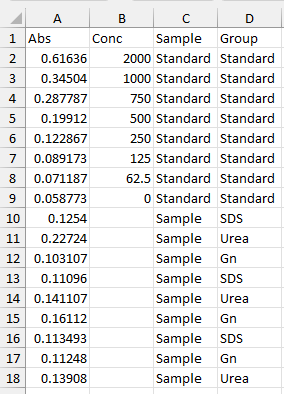
\includegraphics{../Images/exampleexcel.PNG}
\caption{Example excel sheet}
\end{figure}

\pagebreak

\subsubsection{Loading data into
RStudio}\label{loading-data-into-rstudio}

In order to load your data into RStudio you need to first set your
working directory where your file is saved and then use the
\textbf{readxl} package as shown below.

\begin{Shaded}
\begin{Highlighting}[]
\CommentTok{\# Reading in data}

\DocumentationTok{\#\# Load packages}
\FunctionTok{library}\NormalTok{(ggplot2)}
\FunctionTok{library}\NormalTok{(readxl)}
\FunctionTok{library}\NormalTok{(dplyr)}

\DocumentationTok{\#\# Setwd}
\FunctionTok{setwd}\NormalTok{(}\StringTok{"C:/Users/hlajens2/Desktop/Lab work/Protein assays"}\NormalTok{)}

\CommentTok{\# Read in data }
\NormalTok{df }\OtherTok{\textless{}{-}} \FunctionTok{read\_xlsx}\NormalTok{(}\AttributeTok{path =} \StringTok{"Tendon extraction buffer test data.xlsx"}\NormalTok{, }\AttributeTok{sheet =} \DecValTok{3}\NormalTok{) }
\end{Highlighting}
\end{Shaded}

You may need to install the package prior to this but you can do that
with \textbf{install.packages}

After this you need to use your standard to make a linear model for
calculating unknown solutions.

\begin{Shaded}
\begin{Highlighting}[]
\CommentTok{\# Filter for standards}
\NormalTok{df\_standard }\OtherTok{\textless{}{-}}\NormalTok{ df }\SpecialCharTok{\%\textgreater{}\%} 
  \FunctionTok{filter}\NormalTok{(Sample }\SpecialCharTok{==} \StringTok{"Standard"}\NormalTok{)}

\CommentTok{\# Make model}
\NormalTok{model }\OtherTok{\textless{}{-}} \FunctionTok{lm}\NormalTok{(}\AttributeTok{formula =}\NormalTok{ Abs}\SpecialCharTok{\textasciitilde{}}\NormalTok{Conc, }\AttributeTok{data =}\NormalTok{ df\_standard) }

\CommentTok{\# extract coefficients}
\NormalTok{gradient }\OtherTok{\textless{}{-}}\NormalTok{ model}\SpecialCharTok{$}\NormalTok{coefficients[}\DecValTok{2}\NormalTok{] }
\NormalTok{intercept }\OtherTok{\textless{}{-}}\NormalTok{ model}\SpecialCharTok{$}\NormalTok{coefficients[}\DecValTok{1}\NormalTok{] }

\CommentTok{\# plot data}
\NormalTok{df\_standard }\SpecialCharTok{\%\textgreater{}\%} 
  \FunctionTok{ggplot}\NormalTok{(}\FunctionTok{aes}\NormalTok{(}\AttributeTok{x =}\NormalTok{ Conc, }\AttributeTok{y =}\NormalTok{ Abs))}\SpecialCharTok{+}
  \FunctionTok{geom\_point}\NormalTok{()}\SpecialCharTok{+}
  \FunctionTok{geom\_smooth}\NormalTok{(}\AttributeTok{method =} \StringTok{\textquotesingle{}lm\textquotesingle{}}\NormalTok{)}\SpecialCharTok{+}
  \FunctionTok{annotate}\NormalTok{(}\AttributeTok{geom =} \StringTok{\textquotesingle{}text\textquotesingle{}}\NormalTok{,}
           \AttributeTok{x =} \FunctionTok{max}\NormalTok{(df\_standard}\SpecialCharTok{$}\NormalTok{Conc)}\SpecialCharTok{/}\FloatTok{3.4}\NormalTok{, }\CommentTok{\# adjust if placement is off}
           \AttributeTok{y =} \FunctionTok{max}\NormalTok{(df\_standard}\SpecialCharTok{$}\NormalTok{Abs)}\SpecialCharTok{/}\FloatTok{1.3}\NormalTok{, }\CommentTok{\# adjust if placement is off}
           \AttributeTok{label =} \FunctionTok{paste}\NormalTok{(}\StringTok{"Absorbance ="}\NormalTok{,}
                        \FunctionTok{round}\NormalTok{(gradient, }\AttributeTok{digits =} \DecValTok{5}\NormalTok{),}
                        \StringTok{"* Concentration +"}\NormalTok{,}
                        \FunctionTok{round}\NormalTok{(intercept, }\AttributeTok{digits =} \DecValTok{4}\NormalTok{)))}\SpecialCharTok{+}
  \FunctionTok{annotate}\NormalTok{(}\AttributeTok{geom =} \StringTok{\textquotesingle{}text\textquotesingle{}}\NormalTok{,}
           \AttributeTok{x =} \FunctionTok{max}\NormalTok{(df\_standard}\SpecialCharTok{$}\NormalTok{Conc)}\SpecialCharTok{/}\FloatTok{3.4}\NormalTok{, }\CommentTok{\# adjust if placement is off}
           \AttributeTok{y =} \FunctionTok{max}\NormalTok{(df\_standard}\SpecialCharTok{$}\NormalTok{Abs)}\SpecialCharTok{/}\FloatTok{1.4}\NormalTok{, }\CommentTok{\# adjust if placement is off}
           \AttributeTok{label =} \FunctionTok{paste}\NormalTok{(}\StringTok{"Concentration = Absorbance {-} "}\NormalTok{,}
                        \FunctionTok{round}\NormalTok{(intercept, }\AttributeTok{digits =} \DecValTok{4}\NormalTok{),}
                        \StringTok{"/"}\NormalTok{,}
                        \FunctionTok{round}\NormalTok{(gradient, }\AttributeTok{digits =} \DecValTok{5}\NormalTok{)))}

\CommentTok{\# Save graph (This may change depending on directory)}
\FunctionTok{ggsave}\NormalTok{(}\AttributeTok{filename =} \FunctionTok{paste0}\NormalTok{(}\StringTok{"name"}\NormalTok{,}\StringTok{"LOBF"}\NormalTok{, }\StringTok{".png"}\NormalTok{), }
       \AttributeTok{device =} \StringTok{"png"}\NormalTok{,}
       \AttributeTok{dpi =} \DecValTok{600}\NormalTok{,}
       \AttributeTok{path =} \FunctionTok{paste0}\NormalTok{(name, }\StringTok{"/"}\NormalTok{))}
\end{Highlighting}
\end{Shaded}

\begin{figure}
\centering
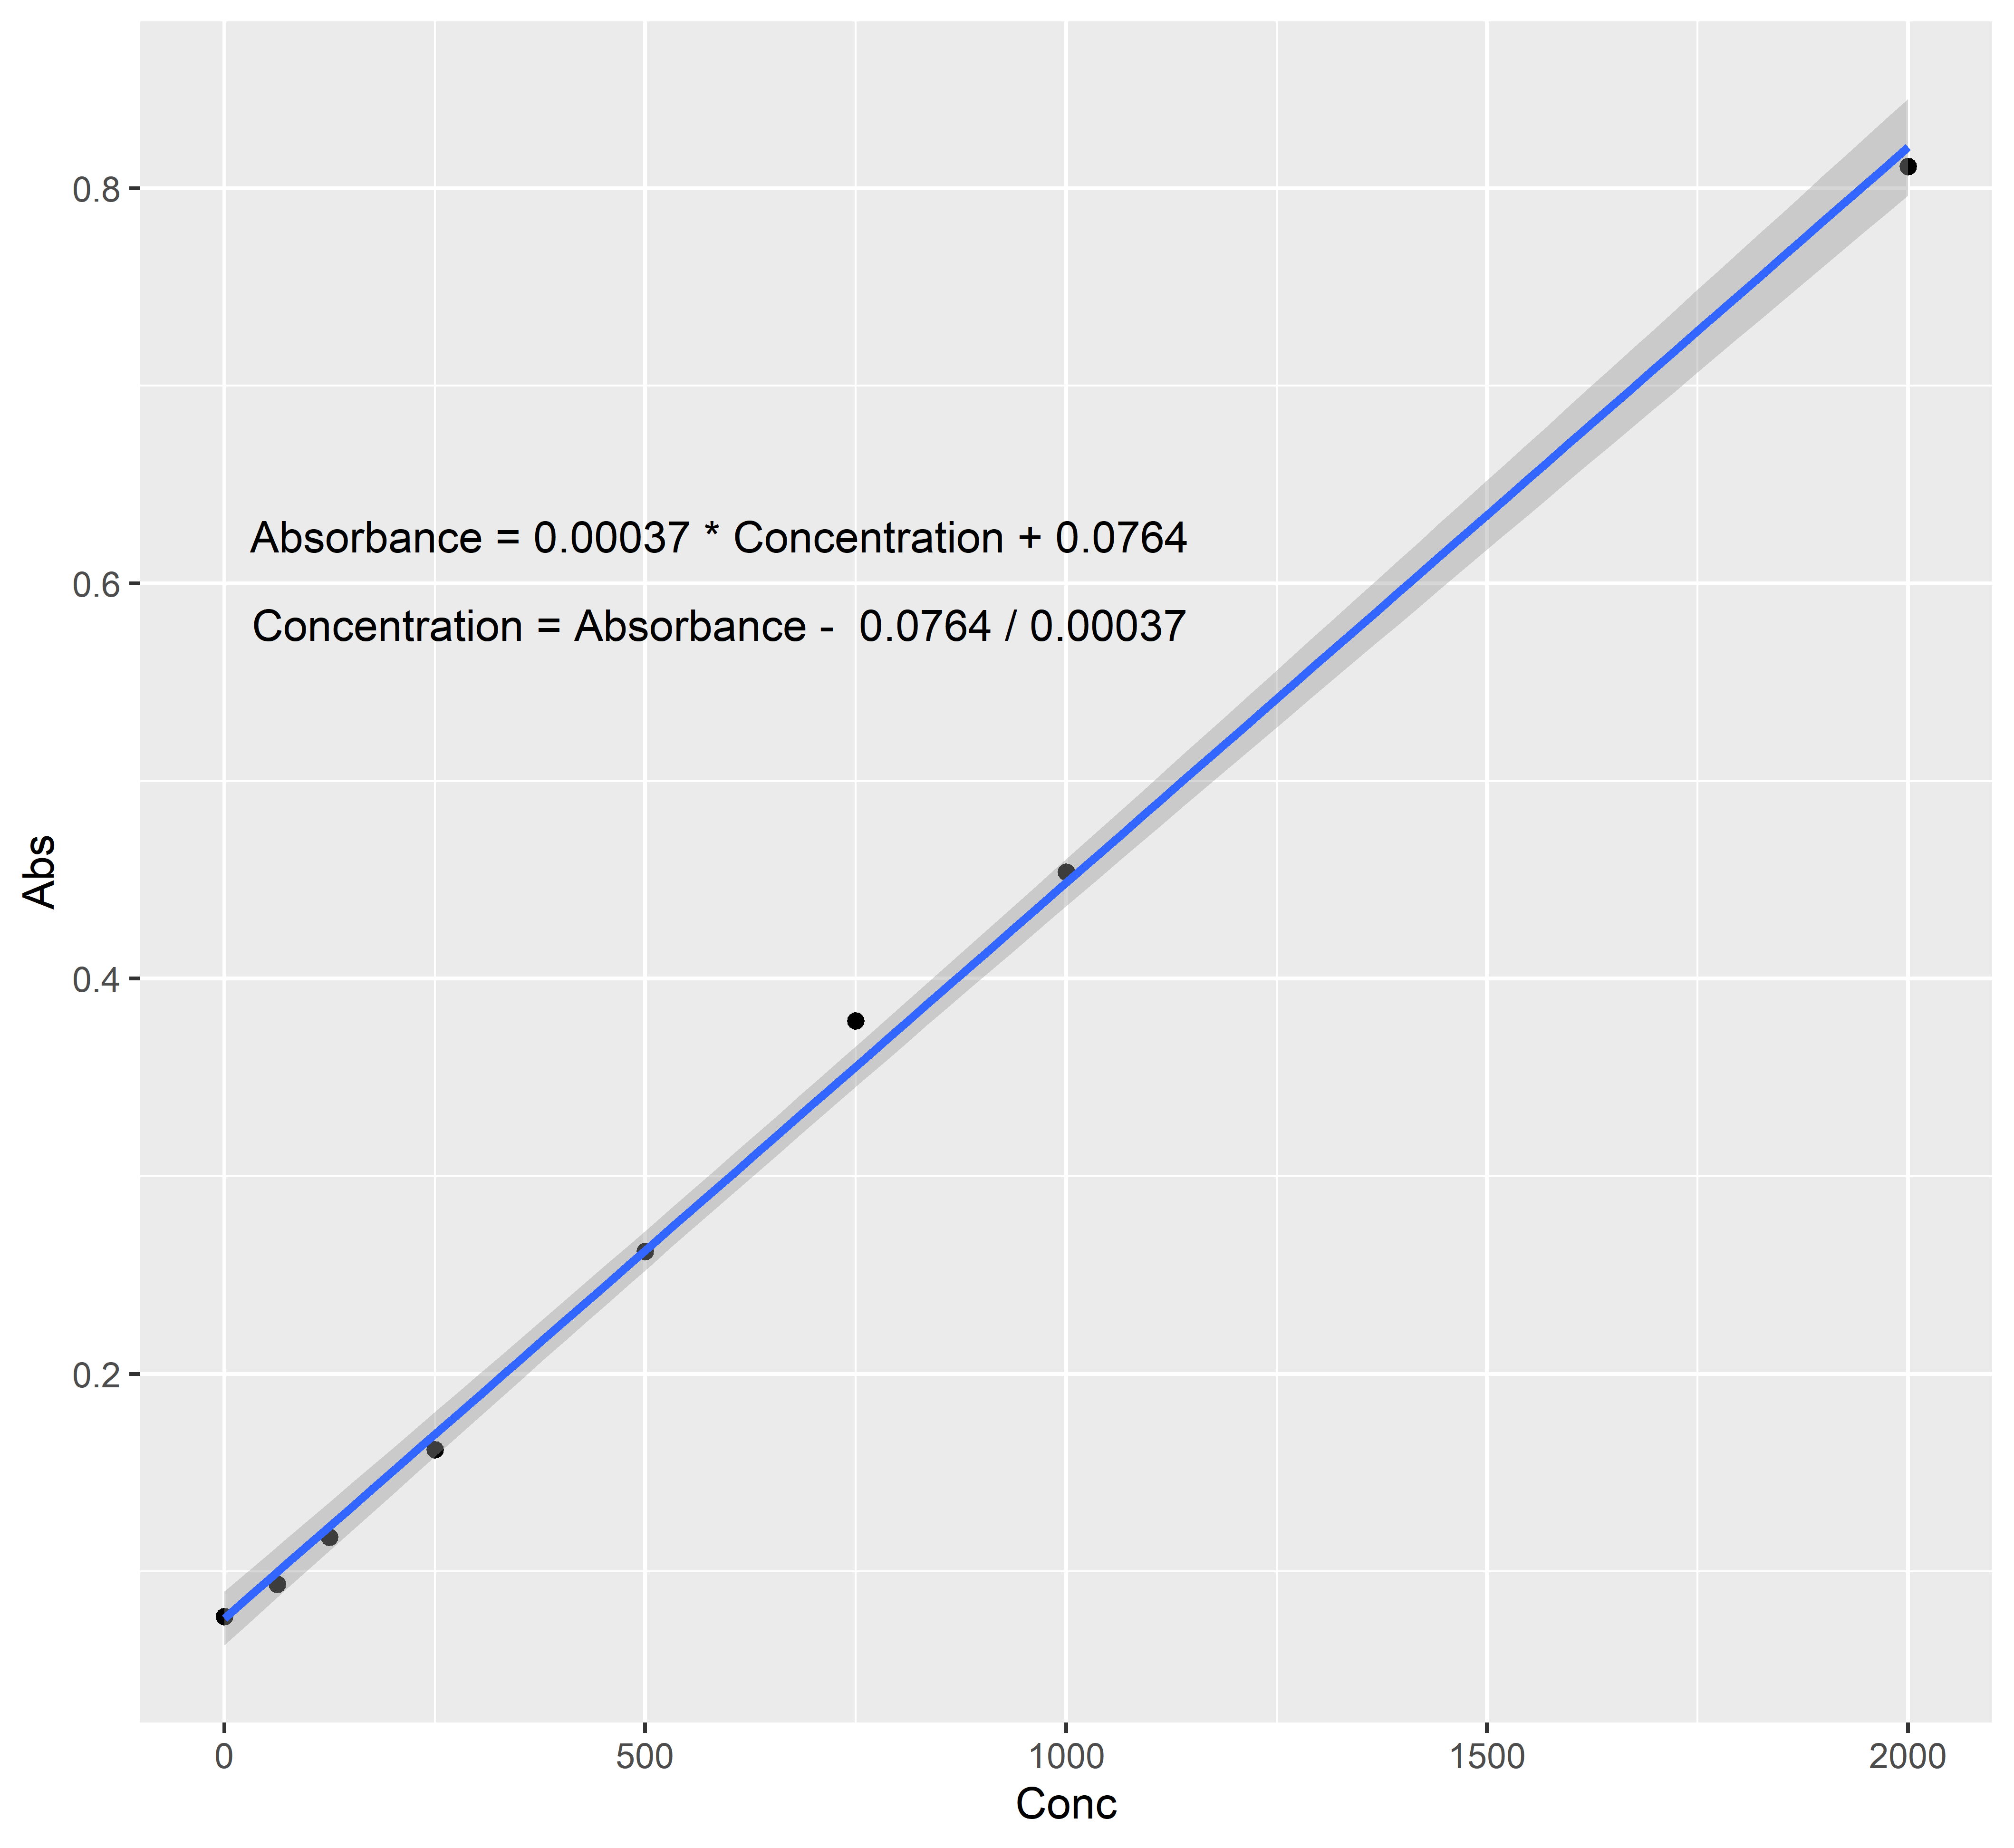
\includegraphics[width=0.8\textwidth,height=\textheight]{../Images/tendon_extraction_testLOBF.png}
\caption{Linear model}
\end{figure}

\pagebreak

Now that you have this information you can begin to work out the unknown
values.

\begin{Shaded}
\begin{Highlighting}[]

\CommentTok{\# Use the model to calculate unknown concentrations}
\NormalTok{df\_samples }\OtherTok{\textless{}{-}}\NormalTok{ df }\SpecialCharTok{\%\textgreater{}\%} 
  \FunctionTok{filter}\NormalTok{(Sample }\SpecialCharTok{==} \StringTok{"Sample"}\NormalTok{) }\SpecialCharTok{\%\textgreater{}\%} 
  \FunctionTok{mutate}\NormalTok{(}\AttributeTok{Conc =}\NormalTok{ (Abs }\SpecialCharTok{{-}}\NormalTok{ intercept)}\SpecialCharTok{/}\NormalTok{gradient)}

\CommentTok{\# Make box plot of data}
\NormalTok{df\_samples }\SpecialCharTok{\%\textgreater{}\%} 
  \FunctionTok{ggplot}\NormalTok{(}\FunctionTok{aes}\NormalTok{(}\AttributeTok{x =}\NormalTok{ Group, }\AttributeTok{y =}\NormalTok{ Conc))}\SpecialCharTok{+}
  \FunctionTok{geom\_boxplot}\NormalTok{(}\FunctionTok{aes}\NormalTok{(}\AttributeTok{fill =}\NormalTok{ Group))}\SpecialCharTok{+}
  \FunctionTok{geom\_jitter}\NormalTok{()}\SpecialCharTok{+}
  \FunctionTok{theme\_classic}\NormalTok{()}\SpecialCharTok{+}
  \FunctionTok{labs}\NormalTok{(}\AttributeTok{x =} \StringTok{"Extraction buffer"}\NormalTok{, }\AttributeTok{y =} \StringTok{"Concentration (ug/mL)"}\NormalTok{)}


\CommentTok{\# Save graph (This may change depending on directory)}
\FunctionTok{ggsave}\NormalTok{(}\AttributeTok{filename =} \FunctionTok{paste0}\NormalTok{(name,}\StringTok{"RES"}\NormalTok{, }\StringTok{".png"}\NormalTok{),}
       \AttributeTok{device =} \StringTok{"png"}\NormalTok{,}
       \AttributeTok{dpi =} \DecValTok{600}\NormalTok{,}
       \AttributeTok{path =} \FunctionTok{paste0}\NormalTok{(name, }\StringTok{"/"}\NormalTok{))}
\end{Highlighting}
\end{Shaded}

\begin{figure}
\centering
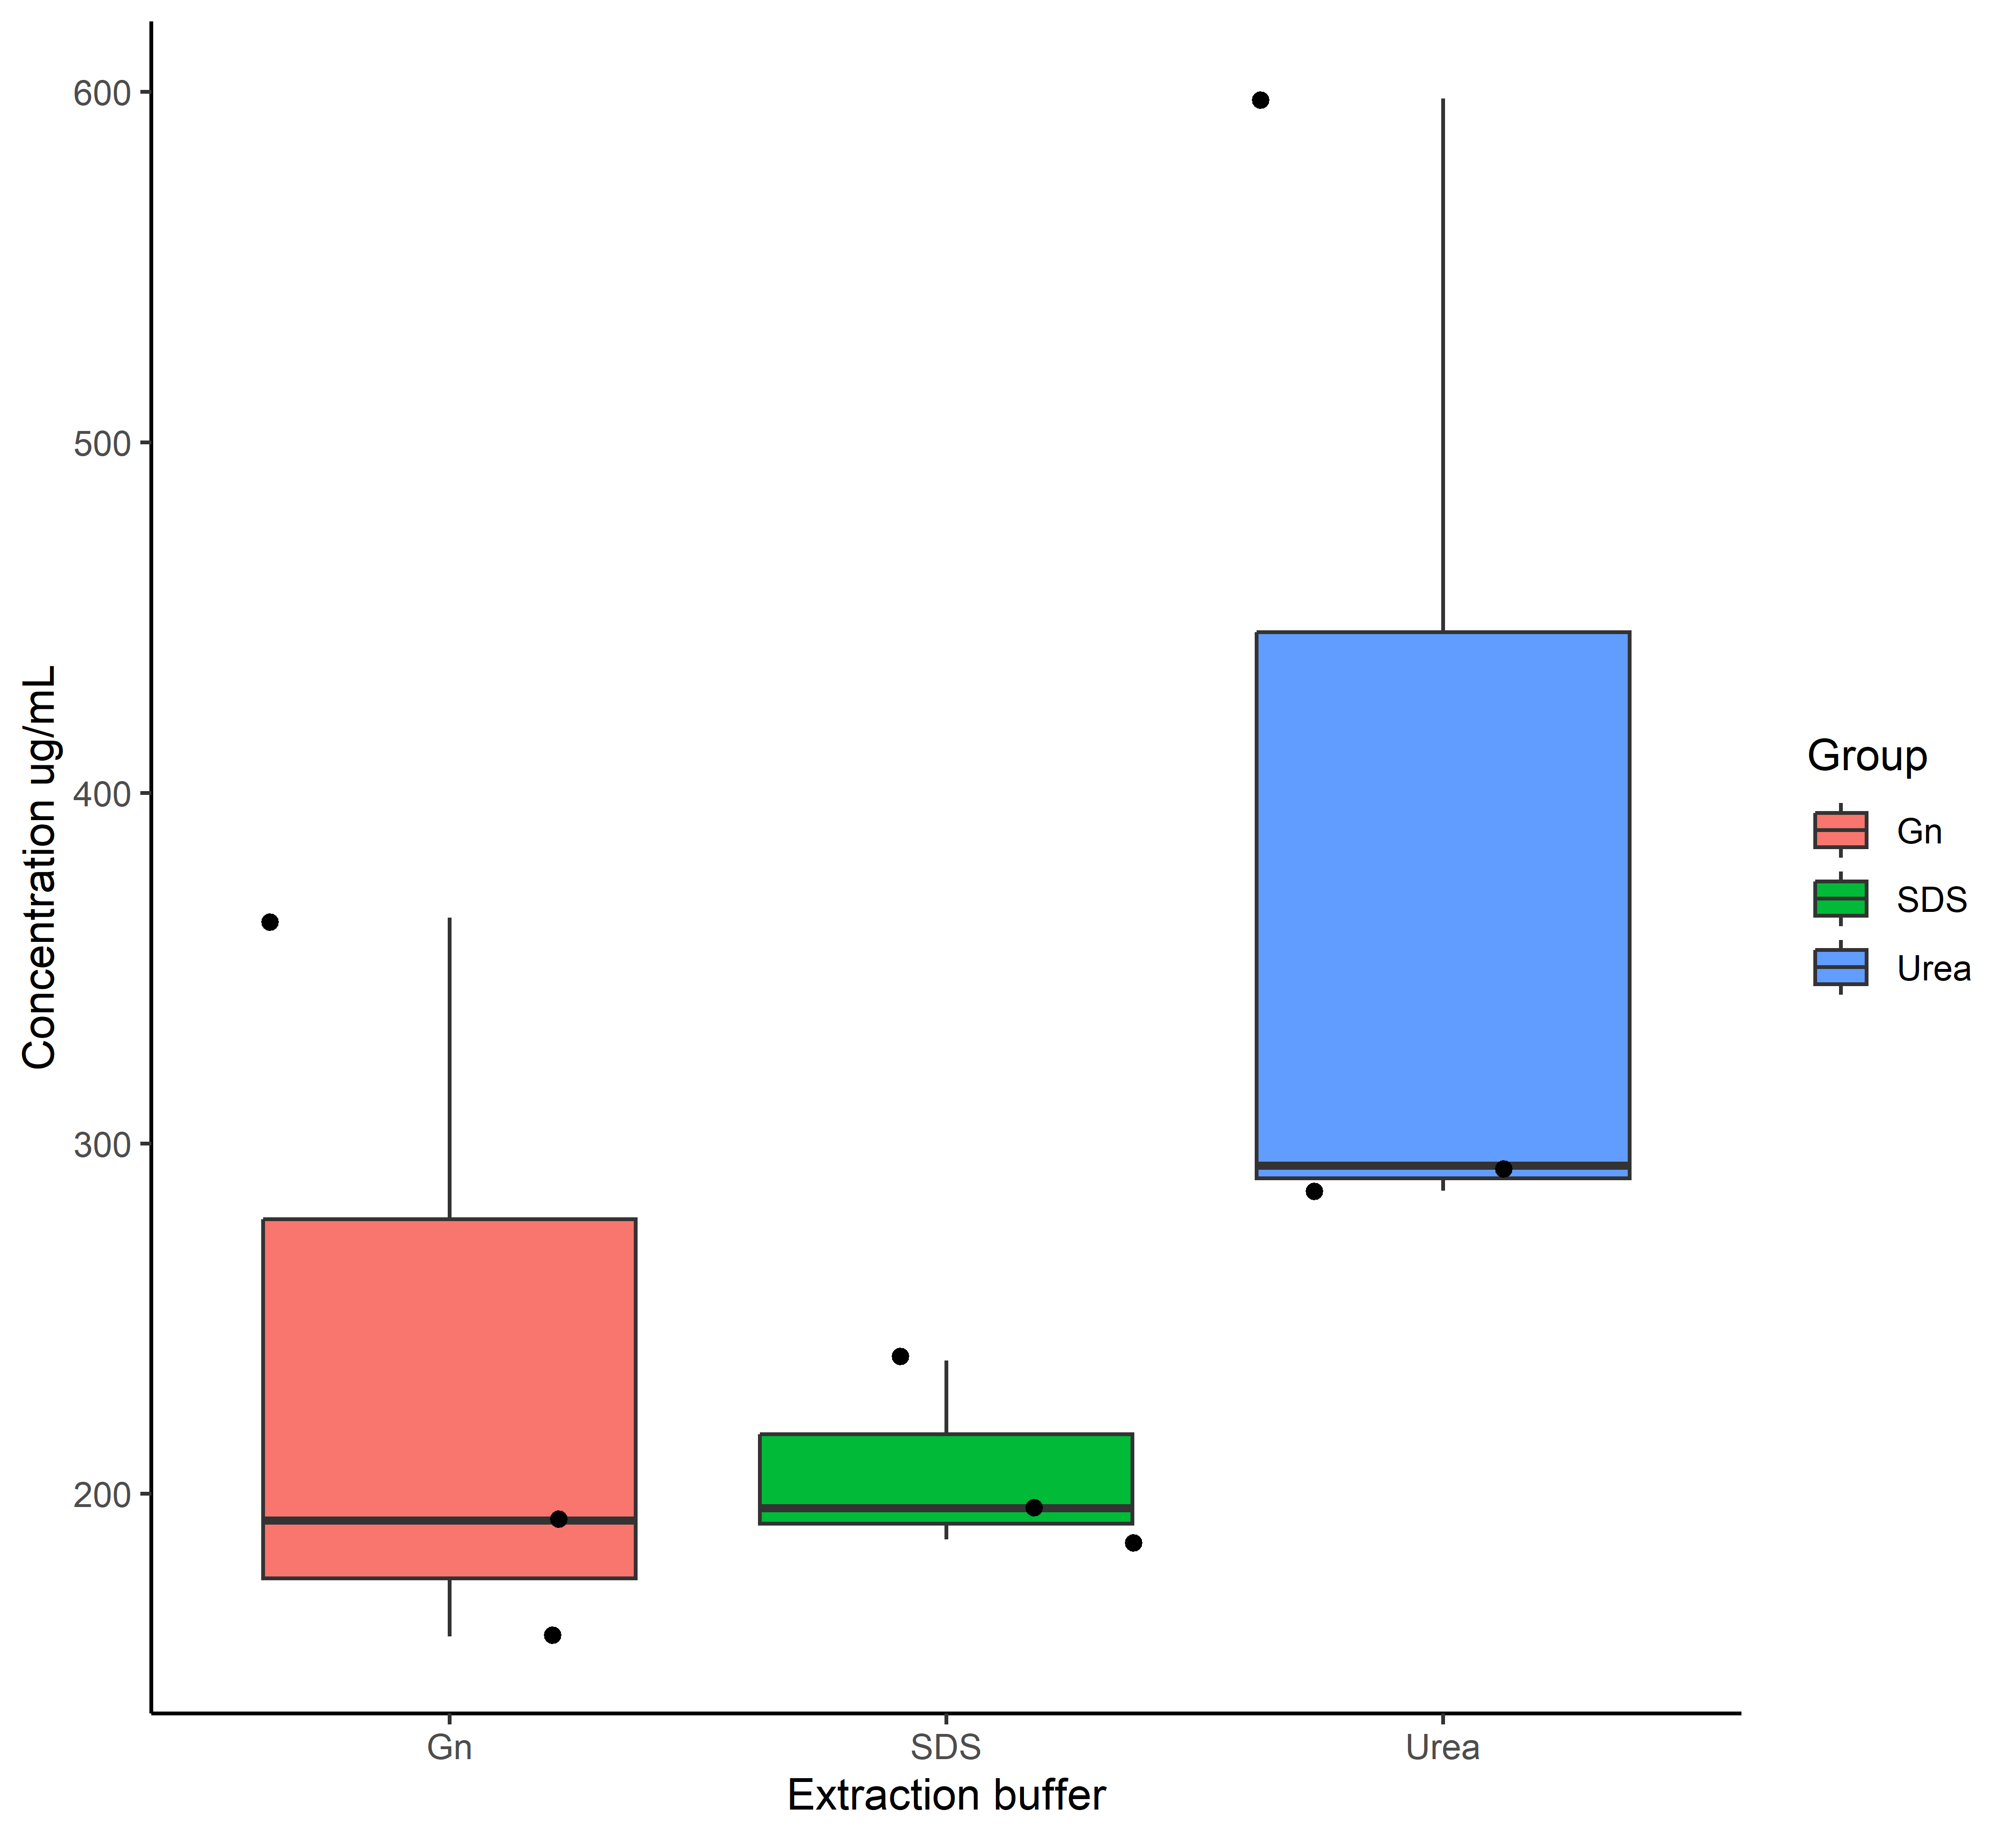
\includegraphics{../Images/tendon_extraction_testRES.png}
\caption{Box plot}
\end{figure}

\pagebreak

The example used in this handbook is a lab experiment testing the effect
of three different extraction buffers on protein extraction. Before
attempting this you need to make sure your data is formatted to suit
your work. If you are having any problems with this or the code is not
working then visit the
\href{https://liverpool-knowhow.libcal.com/appointments/statsliverpool}{KnowHow
page} for more help.

I hope this was useful, there are lots more R tutorials on my
\href{https://ajensen14.github.io/}{website} feel free to email me to
request more RStudio tutorials.

\end{document}
